\documentclass{article}[18pt]
\ProvidesPackage{format}
%Page setup
\usepackage[utf8]{inputenc}
\usepackage[margin=0.7in]{geometry}
\usepackage{parselines} 
\usepackage[english]{babel}
\usepackage{fancyhdr}
\usepackage{titlesec}
\hyphenpenalty=10000

\pagestyle{fancy}
\fancyhf{}
\rhead{Sam Robbins}
\rfoot{Page \thepage}

%Characters
\usepackage{amsmath}
\usepackage{amssymb}
\usepackage{gensymb}
\newcommand{\R}{\mathbb{R}}

%Diagrams
\usepackage{pgfplots}
\usepackage{graphicx}
\usepackage{tabularx}
\usepackage{relsize}
\pgfplotsset{width=10cm,compat=1.9}
\usepackage{float}

%Length Setting
\titlespacing\section{0pt}{14pt plus 4pt minus 2pt}{0pt plus 2pt minus 2pt}
\newlength\tindent
\setlength{\tindent}{\parindent}
\setlength{\parindent}{0pt}
\renewcommand{\indent}{\hspace*{\tindent}}

%Programming Font
\usepackage{courier}
\usepackage{listings}
\usepackage{pxfonts}

%Lists
\usepackage{enumerate}
\usepackage{enumitem}

% Networks Macro
\usepackage{tikz}


% Commands for files converted using pandoc
\providecommand{\tightlist}{%
	\setlength{\itemsep}{0pt}\setlength{\parskip}{0pt}}
\usepackage{hyperref}

% Get nice commands for floor and ceil
\usepackage{mathtools}
\DeclarePairedDelimiter{\ceil}{\lceil}{\rceil}
\DeclarePairedDelimiter{\floor}{\lfloor}{\rfloor}

% Allow itemize to go up to 20 levels deep (just change the number if you need more you madman)
\usepackage{enumitem}
\setlistdepth{20}
\renewlist{itemize}{itemize}{20}

% initially, use dots for all levels
\setlist[itemize]{label=$\cdot$}

% customize the first 3 levels
\setlist[itemize,1]{label=\textbullet}
\setlist[itemize,2]{label=--}
\setlist[itemize,3]{label=*}

% Definition and Important Stuff
% Important stuff
\usepackage[framemethod=TikZ]{mdframed}

\newcounter{theo}[section]\setcounter{theo}{0}
\renewcommand{\thetheo}{\arabic{section}.\arabic{theo}}
\newenvironment{important}[1][]{%
	\refstepcounter{theo}%
	\ifstrempty{#1}%
	{\mdfsetup{%
			frametitle={%
				\tikz[baseline=(current bounding box.east),outer sep=0pt]
				\node[anchor=east,rectangle,fill=red!50]
				{\strut Important};}}
	}%
	{\mdfsetup{%
			frametitle={%
				\tikz[baseline=(current bounding box.east),outer sep=0pt]
				\node[anchor=east,rectangle,fill=red!50]
				{\strut Important:~#1};}}%
	}%
	\mdfsetup{innertopmargin=10pt,linecolor=red!50,%
		linewidth=2pt,topline=true,%
		frametitleaboveskip=\dimexpr-\ht\strutbox\relax
	}
	\begin{mdframed}[]\relax%
		\centering
		}{\end{mdframed}}



\newcounter{lem}[section]\setcounter{lem}{0}
\renewcommand{\thelem}{\arabic{section}.\arabic{lem}}
\newenvironment{defin}[1][]{%
	\refstepcounter{lem}%
	\ifstrempty{#1}%
	{\mdfsetup{%
			frametitle={%
				\tikz[baseline=(current bounding box.east),outer sep=0pt]
				\node[anchor=east,rectangle,fill=blue!20]
				{\strut Definition};}}
	}%
	{\mdfsetup{%
			frametitle={%
				\tikz[baseline=(current bounding box.east),outer sep=0pt]
				\node[anchor=east,rectangle,fill=blue!20]
				{\strut Definition:~#1};}}%
	}%
	\mdfsetup{innertopmargin=10pt,linecolor=blue!20,%
		linewidth=2pt,topline=true,%
		frametitleaboveskip=\dimexpr-\ht\strutbox\relax
	}
	\begin{mdframed}[]\relax%
		\centering
		}{\end{mdframed}}
\lhead{Computer Systems}
\usepackage{calc}
\usepackage{amsmath}
\usepackage{array}
\usepackage{xlop}

\begin{document}
\begin{center}
\underline{\huge Binary Arithmetic and Floating point}
\end{center}
\section{Binary Addition}
$$
\begin{array}{r}
\phantom{0}111\phantom{000}\\				
\phantom{00}11100\\
\underline{\mbox{} +\phantom{0}01110}\\
\phantom{0}101010
\end{array}
$$
\section{Overflow}
Suppose the accumulator in your CPU is an 8 bit register\\
It has 11010010 in it\\
You execute the instruction ADD 01010000\\
What happens?
$$
\begin{array}{r}			
\phantom{0}11010010\\
\underline{\mbox{} +01010000}\\
100100010
\end{array}
$$
The answer \textbf{doesn't fit} in the register. This should trigger a flag in the \textbf{status register}, but can cause errors
\section{Binary Multiplication}
$$
\begin{array}{r}			
\phantom{0000}11100\\
\underline{\mbox{}\times 01110}\\
\phantom{0000}00000\\
\phantom{000}111000\\
\phantom{00}1110000\\
\phantom{0}11100000\\
\underline{000000000}\\
110001000
\end{array}
$$
This can be efficiently accomplished with \textbf{left-shift} and \textbf{add} operations
\section{Negative Numbers}
\textit{How can we represent \textbf{negative numbers using only bits?}}\\
Common Solutions:
\subsection{Signed Magnitude Representation}
\begin{itemize}
\item Add a single bit flag: 0 for positive or 1 for negative
\begin{itemize}
\item \textbf{0}000 0110=6
\item \textbf{1}000 0110=-6 (Not 134)
\end{itemize}
\item Similar in concept to a minus sign
\item Have two values for 0: 1000 0000 and 0000 0000
\item Makes binary arithmetic messy
\end{itemize}
\subsection{Ones Compliment}
\begin{itemize}
\item The negative of a number is represented by flipping each bit
\item For example 0100 1001=65 becomes 1011 0110=-65
\item The higher order bit still indicates the sign of the number
\item Still has two representations for zero: 00000000 and 11111111
\item Makes binary addition a bit simpler
\item Due to this method, only get 7 bits of data in a byte
\end{itemize}
\subsection{Twos Compliment}
\begin{itemize}
\item A negative number is obtained by flipping each bit and adding 1
\item For example 0100 1001=65 becomes 1011 0111=-65
\item The higher order bit still indicates the sign of the number
\item One representation for 0: 00000000
\item Makes binary arithmetic much simpler
\item Allows counting by addition in the way you would expect
\end{itemize}
\subsection{Add a bias}
\begin{itemize}
\item For k-bit numbers add a bias of $2^{k-1}-1$ then store in normal binary (So for 8-bit add $2^7-1=127$
\item Can store numbers between $-(2^{k-1}-1)$ and $2^{k-1}$ (-127 and 128)
\item For example -65 stored as -65+127=62 becomes 0011 1110
\item The higher order bit \textbf{does not indicate} the sign of the number in the normal way
\item Used in storing floating point numbers for some reason
\end{itemize}
\subsection{More on Twos compliment}
We will stick with \textbf{twos compliment}\\
We need to be careful about how many bits we are using to represent a number:\\
In this method, the leading zeros are important, and so cannot be ignored
\\
\begin{tabular}{l l l}
4 Bits:&$3_{10}=0011_2$&$-3_{10}=1101_2$\\
8 Bits:&$3_{10}=0000 0011_2$&$-3_{10}=1111 1101_2$
\end{tabular}\\
\\
Subtracting is now the same as adding: 10-3=10+(-3)\\
$10_{10}=0000 1010_2, 3_10=0000 0011_2$\\
$0000 1010 - 0000 0011=0000 1010 + 1111 1101=1 0000 0111$ (Overflow so $0000 0111$)\\
\\
Note that 10000000 is it's own negative, but is taken to be -128
\section{Floating point representation}
Sometimes we need to deal with numbers outside the usual range:\\
\\
\textbf{Floating point} is very like scientific notation\\
The typical floating point representation has three fields:\\
\begin{tabular}{l l}
The sign bit& S\\
The exponent& e\\
The mantissa& M (Also called the significand)
\end{tabular}\\
These are used to represent the number:
$$\textrm{+ or - } M \times2^e$$
Single precision (32 bit) floating point numbers have:
\begin{itemize}
\item 1 bit sign
\item 8 bit exponent
\item 23 bit mantissa
\end{itemize}
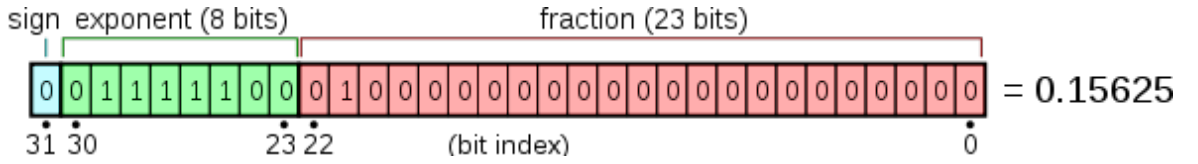
\includegraphics[width=\textwidth]{float.png}
\subsection{The sign bit, S}
0 indicates a positive number\\
1 indicates a negative number
\subsection{The exponent, e}
Value in range -126 to 127\\
Stored with a \textbf{bias}: 127 is added giving a number between 1 and 254\\
\\
The 8 bit exponent field can store values in the range 0 to 255, but 0 and 255 have \textbf{special meanings}:
\begin{itemize}
\item Exponent field 0 with mantissa 0 gives the number 0
\item Exponent field 0 with a non-zero mantissa: "subnormal numbers" - below the threshold of numbers normally dealt with in floating point representation
\item Exponent field 255 with mantissa 0 gives + or - infinity
\item Exponent field 255 with non-zero mantissa: not a number
\end{itemize}
\subsection{The mantissa, M}
Some binary number like 1.10101010110\\
Always scaled so that the radix point is after the leading 1\\
Hence we need not store the leading 1 (we can assume it is there)\\
We only store 23 bits of the fractional part
\subsection{Example}
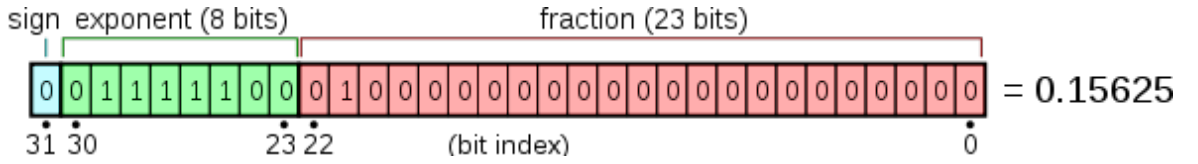
\includegraphics[width=\textwidth]{float.png}
\begin{itemize}
\item Sign 0 - a positive number
\item Exponent field is 124, so e is 124-127=-3
\item Mantissa field is 010... so the actual mantissa is calculated to 1.25
\item $1.25\times2^{-3}=1.25/8=0.15625$
\end{itemize}
\subsection{Example 2}
-12.375\\
$12.375_{10}=1100.011_2$\\
$1100.011 = 1.100011\times 2^3$
\begin{itemize}
\item Sign is 1 to represent a negative
\item Mantissa is 1.100011, we will store 100011000...
\item Exponent is 3, we will store $130_{10}=1000 0010_2$ after adding the bias of 127. Exponent is 3 to shift the radix point 3 places to the left so that the number starts 1. etc
\end{itemize}
11000001010001100000000000000000
\subsection{More on floating point}
\subsubsection{Error in truncation}
What is the binary FP representation of $0.1_{10}$?\\
$0.1_{10} = 0.0001100110011001100110011…_2$\\
So the FP has e = -4; M = 1.10011001100110011001101 (limited to 23 digits)\\
which is actually 0.100000001490116119384765625, this is a \textbf{rounding error}.\\
\subsubsection{Error in overflow/underflow}
Minimum positive number is $2^{-126}$, the \textbf{underflow level}.\\
Maximum positive number is ($2-2^{-23}$) $\times 2^{127}$, the \textbf{overflow level}.\\
\\
Floating Point Operations should return the closest FP number to the answer. E.g. $1.1\times2^{123} – 1.10101\times2^{-23} = 1.1\times2^{123}$. In this the number being subtracted is too small to make a difference to such a large number

\end{document}